\documentclass[10pt,a4paper]{article}

\usepackage{indentfirst}
%\usepackage{arev}
\usepackage{amsthm,amsfonts,amsmath,amssymb}
\usepackage[brazilian]{babel}
\usepackage[T1]{fontenc}
%\usepackage[latin1]{inputenc}
\usepackage[utf8]{inputenc}
%\usepackage{multicol}
\usepackage{setspace}
%\usepackage{natbib}
\usepackage[usenames,dvipsnames]{xcolor} 
\usepackage{pgf,tikz}
%\usepackage{algpseudocode}
\usepackage{float}
\usepackage{graphicx}
\usepackage{subfigure}
\usepackage{wrapfig}
%\usepackage{listings}
%\usepackage[linesnumbered, ruled, portuguese]{algorithm2e}
\usepackage{multirow}
%\usepackage{verbatim}
%\usepackage[active,tightpage]{preview}
%\PreviewEnvironment{tikzpicture}
%\setlength\PreviewBorder{5pt}
\usepackage{geometry}
\usepackage[pdftex]{hyperref}
\usepackage{listings}
\usepackage[normalem]{ulem}
\usepackage{caption}
\geometry{a4paper,inner=2.0cm,outer=2.0cm,top=2.0cm,bottom=2.0cm}


\newcommand{\pr}{\hspace*{0.6cm}}
\newcommand{\vesp}{\vspace*{.3cm}}

\newcommand{\sen}{\mbox{\,sen}}
\newcommand{\cotg}{\mbox{\,cotg\,}}
\newcommand{\tg}{\mbox{\,tg\,}}
\newcommand{\cose}{\mbox{\,cos\,}}
\newcommand{\expo}{\mbox{\,e\,}}
\newcommand{\logg}{\mbox{\,log}}
\newcommand{\Sum}{\displaystyle\sum}
\newcommand{\Prod}{\displaystyle\prod}
\newcommand{\Int}{\displaystyle\int}
\newcommand{\dint}{\, \mathrm{d}}
\newcommand{\Lim}{\displaystyle \lim}
\newcommand{\Frac}{\displaystyle\frac}

\newcommand{\Nc}{N_{cont}}
\newcommand{\Ni}{N_{int}}
\newcommand{\Ne}{N_{estrela}}

\newcommand{\Dparc}[2]{\dfrac{\partial #1}{\partial #2}}
\newcommand{\Dparcn}[3]{\dfrac{\partial^#3 #1}{\partial^#3 #2}}

\newcommand{\R}{\mathbb{R}}
\newcommand{\V}{\mathcal{V}}
\newcommand{\I}{I_u}
\newcommand{\Fi}{\varphi}
\newcommand{\se}{\mbox{ se }}
\newcommand{\norma}[1]{\left|\left| #1 \right|\right|}
\newcommand{\sistema}[1]{ \left\{ #1 \right. }

\newtheorem{exemplo}{\pr \sc Exemplo}[section]%[chapter]
\newtheorem{defi}{\pr \sc Defini\c{c}\~ao}[section]%[chapter]
\newtheorem{obs}{\pr \sc Observa\cao}[section]%[chapter]
\newtheorem{teor}{\pr \sc Teorema}[section]%[chapter]
\newtheorem{lema}{\pr \sc Lema}[section]%[chapter]
\newtheorem{prop}{\pr \sc Proposi\cao}[section]%[chapter]
\newtheorem{exercise}{\pr \sc Exerc\'\i cios}[section]%[chapter]
\newtheorem{alg}{\pr Algoritmo}[section]%[chapter]

\setlength{\columnsep}{1cm}

\setlength{\columnsep}{1cm}

%basicstyle=\footnotesize\ttfamily,


\begin{document}

\thispagestyle{empty}
\begin{center}
	UNIVERSIDADE DE SÃO PAULO – USP
	
	INSTITUTO DE CIÊNCIAS MATEMÁTICAS E DE COMPUTAÇÃO
	
	DEPARTAMENTO DE SISTEMAS DE COMPUTAÇÃO
	
	\vspace{7cm}
	
	\Large{\textbf{TORRES DE HANÓI}}
	
	\vspace{6cm}
	
    \textbf{Alunos:}\\
	Adams Vietro Codignotto da Silva - $6791943$ \\ 
    Ana Clara Kandratavicius Ferreira - $7276877$\\
    Frederico Facco - $8532206$\\
	 
	\vspace{6cm}
	
	São Carlos
	
	2014
\end{center}

\newpage

\pagenumbering{arabic}

\section{Introdução}
Neste trabalho, iremos resolver o famoso problema das Torres de Hanói, utilizando uma representação em grafo e técnicas aprendidas em IA.
\section{Modelagem do problema}
A meta é obter o número mínimo de movimentos. O número mínimo pode ser obtido utilizando recorrência.

Tomando \textit{n} como número de discos, \textit{a}, \textit{b} e \textit{c} como os pinos e $H(n,a,b,c)$ como a quantidade de movimentos para passar do pino \textit{a} para o pino \textit{b}, utilizando o auxiliar \textit{c}, temos:
\begin{equation}
\nonumber
\begin{array}{l}
H(1,a,b,c) = 1 \quad (a \rightarrow c)\\
H(n,a,b,c) = H(n-1,a,b,c), \quad (a \rightarrow b), H(n-1,c,b,a)
\end{array}
\end{equation}
Podemos dizer então que para um número \textit{n} de discos, podemos gerar um grafo contendo todas as possibilidades, com $3^n$ nós.
\begin{figure}[H]
\centering
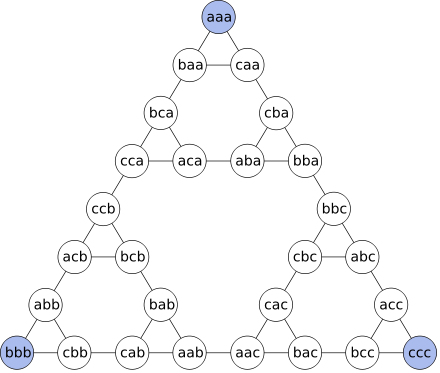
\includegraphics[scale=0.5]{1.png}
\caption*{\small{Grafo de possibilidades com 3 discos}}
\end{figure}
\subsection{Recorrência}
Podemos dividir o problema da Torre de Hanói de acordo com o número de discos:
\begin{itemize}
\item Para n=1, basta 1 movimento
\item Para n=2, precisamos de 3 movimentos (trivial)
\item Para n=3, podemos resolver o problema para 2 discos (3 movimentos), mover o disco maior para o pino restante (1 movimento), e movemos os outros 2 discos para o pino final (3 movimentos) totalizando 7 movimentos.
\item Para n=4, Resolvemos o problema para três discos(7 movimentos), depois movemos o maior disco (1 movimento), após isso trazemos os três discos que já estão no outro pino para cima do maior disco (7 movimentos), totalizamos 15 movimentos.
\end{itemize}
Podemos perceber que temos a seguinte seqüencia:
\begin{itemize}
\item $1=2^1 -1$
\item $3=2^2 -1$
\item $7=2^3 -1$
\item $15=2^4 -1$
\end{itemize}
Ou seja, temos $2^n-1$ movimentos necessários para uma quantidade \textit{n} de pinos.

\section{Implementação}
O problema foi implementado na linguagem C. Para compilação, pode ser usado o comando make all no terminal de um sistema Linux, utilizando o arquivo makefile presente, e executar utilizando o comando make run. No Windows, uma alternativa é utilizar um compilador como o CodeBlocks, criar um projeto, incluir todos os arquivos .c e .h e compilar normalmente.
\subsection{Entrada}
Como entrada, apenas é preciso digitar o número de discos a serem utilizados (variando de 1 a 20). Mais que 20 discos são possíveis, mas devido a grande quantidade de memória e processamento utilizado, não é recomendável, além de tornar o programa instável.
\subsection{Saída}
A saída exibirá a quantidade de estados (nós) que o BFS e o DFS visitaram, e o caminho que ambos encontraram. Após isso, irá mostrar os estados a serem executados pelo A*, ou seja, os vértices visitados do grafo, onde haverão k linhas representando os k-1 movimentos (pois a primeira é o estado inicial) com n números variando de 1 a 3, onde n é a quantidade de discos desejados. Cada número representa em qual pino o disco deve estar presente na jogada k, ou seja, uma saída \textit{1 3} quer dizer que o disco 1 deve estar no pino 1 e o disco 2 deve estar no pino 3.

\subsection{Estruturas}
Para representar tal grafo, foi utilizado uma representação de grafo com listas de adjacências para conservar memória.

Também foram implementadas estruturas adicionais necessárias, como uma fila de prioridade e uma pilha.

\subsection{Buscas Cegas}
Utilizamos o algoritmo de buscas DFS e BFS como buscas cegas, pois são métodos mais comuns e simples de serem implementados, além de percorrerem todo o grafo.

\subsection{Heurísticas}
Para percorrer o grafo eficientemente, utilizamos o algoritmo A*. Como heurísticas, utilizamos duas funções:
\begin{itemize}
\item Um contador de movimentos, onde a cada estado que passamos é incrementado.
\item A distância do estado até o estado desejado, onde o peso atribuído ao nó é a quantidade de discos que ainda não estão na posição final (no terceiro pino)
\end{itemize}
\section{Experimentos e Resultados}
O algoritmo A* se mostra bem próximo do ideal, como podemos observar pela tabela abaixo, onde mostra a quantidade de nós visitados.
\begin{center}
\begin{table}[H]
\begin{tabular}{|c|c|c|c|c|}
\textbf{Número de Discos} & \textbf{BFS} & \textbf{DFS} & \textbf{A*} & \textbf{Ideal} \\
\hline
1 & 1 & 1 & 1 & 1 \\
2 & 6 & 8 & 3 & 3 \\
3 & 24 & 26 & 8 & 7\\
4 & 70 & 74 & 15 & 15\\
5 & 232 & 220 & 25 & 24\\
\end{tabular}
\end{table}
\end{center}
Porém, o A* necessita de quase 3 vezes mais memória que o DFS ou o BFS, pois necessita guardar o peso de todos os vértices, bem como seus antecessores e se já foram visitados.
\section{Conclusões}
Para este problema, em particular para o modo em que foi modelado, o algoritmo DFS sempre encontrará a solução ideal. Porém, o algoritmo A* se mostrou muito mais eficiente em questão de nós visitados, mesmo às vezes não exibindo a solução ideal.

Talvez o uso de outra linguagem orientada a objeto, como C++ ou Python, tornaria o código mais limpo e de fácil entendimento. Mas como todos os integrantes possuem maior afinidade com C, esta foi a linguagem escolhida.
\end{document}
